\documentclass[9pt, aspectratio=169]{beamer}
\usepackage{FiraSans}
\usetheme[subsectionpage=progressbar]{metropolis}
\usepackage[utf8]{inputenc}
\usepackage{amsmath}
\usepackage{amsfonts}
\usepackage{amssymb}
\usepackage{multicol}
\usepackage{tikz}
\usepackage{caption}
\usepackage{xcolor}
\usepackage[T1]{fontenc} 
\usepackage[skins]{tcolorbox}
\author{Nicola Roman\`o - nicola.romano@ed.ac.uk}
\title{Lecture 11 - Convolutional Neural Networks (CNN)}
\setlength{\fboxsep}{0pt}
\setbeamertemplate {footline}{\begin{scriptsize}\hfill\insertframenumber ~of \inserttotalframenumber\kern1em\vskip5pt\end{scriptsize}}

% Remove "Figure" in front of captions
% See https://tex.stackexchange.com/questions/82456/how-to-remove-figure-caption-prefix-figure-in-beamer
\captionsetup{labelformat=empty,labelsep=none}

\titlegraphic{\centering 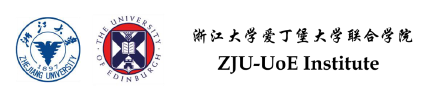
\includegraphics[scale=.5]{instituteLogo.png}}
\date{}

\begin{document}

\newtcolorbox{codebox}{enhanced,
    top=2pt,
    left=2pt,
    right=2pt,
    bottom=2pt,
    boxrule=0pt,
    leftrule=5pt,
    sharp corners,
    colback=gray!20,
    colframe=blue!60!black}

\begin{frame}
    \titlepage
\end{frame}

\begin{frame}
    {Learning objectives}
    \begin{columns}
        \begin{column}{0.8\textwidth}
            \begin{itemize}
                \item LO 1
                \item LO 2
                \item LO 3
            \end{itemize}
        \end{column}
        \begin{column}{0.2\textwidth}
            
\includegraphics[angle=-30, origin=tr, width=1.5\textwidth]{lightbulb.png}
        \end{column}
    \end{columns}
\end{frame}

\section{Introduction}

\begin{frame}
    {From shallow to deep networks}
    In Lecture 11 we introduced neural networks. With increasing depth, neural networks can solve more complex problems.
    This comes at the cost of increased computational complexity (more parameters to learn).
    \vspace{1em}

    \begin{columns}[T]
        \begin{column}{.3\textwidth}
            \textbf{McCulloch-Pitts neuron}
            \vspace{2em}

            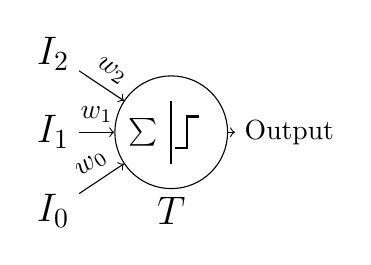
\begin{tikzpicture}[scale=1]
                % Neuron
                \node [draw, fill=white, circle, minimum height=4em] (n) at(1.5, 1) {$\sum\qquad$};
                \node [below of = n] {\Large\textbf{$T$}};

                % Inputs and weights
                \foreach \i in {0,1,2}
                    {
                        \node (i\i) at(0,\i) {\Large$I_\i$};
                        \draw [->] (i\i) -- node [above, midway, sloped] {\textbf{$w_\i$}} (n);
                    }

                \node (out) at(3, 1) {Output};
                \draw [->] (n) -- (out);
                \draw [thick] (1.5, .6) -- (1.5, 1.4);

                \draw [thick] (1.55, 0.8) -- (1.7, 0.8) -- (1.7, 1.2) -- (1.85, 1.2);
            \end{tikzpicture}
        \end{column}
        \begin{column}{.3\textwidth}
            \textbf{Single layer perceptron}
            \vspace{2em}

            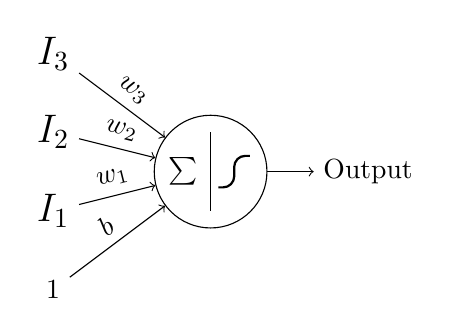
\begin{tikzpicture}
                % Neuron
                \node [draw, fill=white, circle, minimum height=4em] (n) at(2, 1.5) {$\sum\qquad$};

                % Bias
                \node (b) at(0, 0) {1};
                \draw [->] (b) -- node [above, midway, sloped] {\textbf{$b$}} (n);

                % Inputs and weights
                \foreach \i in {1,2,3}
                    {
                        \node (i\i) at(0,\i) {\Large$I_\i$};
                        \draw [->] (i\i) -- node [above, midway, sloped] {\textbf{$w_\i$}} (n);
                    }

                \node (out) at(4, 1.5) {Output};
                \draw [->] (n) -- (out);

                % Activation function
                \draw [thick, rounded corners] (2.1, 1.3) -- (2.3, 1.3) -- (2.3, 1.7) -- (2.5, 1.7);

                \draw (2, 1) -- (2, 2);
            \end{tikzpicture}
        \end{column}
        \begin{column}{.3\textwidth}
            \textbf{Multi-layer perceptron}
            \vspace{2em}

            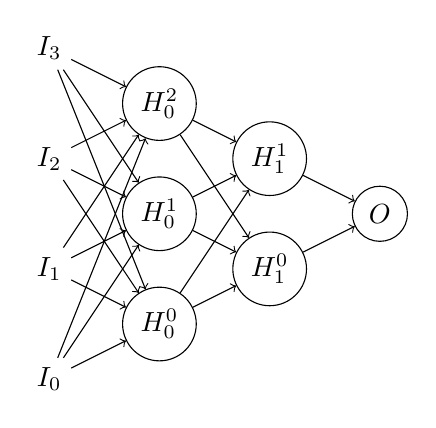
\begin{tikzpicture}[scale=.7]
                \tikzstyle{unit}=[draw,fill=white,shape=circle,minimum size=.7cm]

                \node (x0) at (0,0){$I_0$};
                \node (x1) at (0,2){$I_1$};
                \node (x2) at (0,4){$I_2$};
                \node (x3) at (0,6){$I_3$};

                \node[unit](h0) at (2,1){$H_0^0$};
                \node[unit](h1) at (2,3){$H_0^1$};
                \node[unit](h2) at (2,5){$H_0^2$};

                \node[unit](h3) at (4,2){$H_1^0$};
                \node[unit](h4) at (4,4){$H_1^1$};

                \node[unit](o) at (6,3){$O$};

                \draw[->] (x0) -- (h0);
                \draw[->] (x1) -- (h0);
                \draw[->] (x2) -- (h0);
                \draw[->] (x3) -- (h0);
                \draw[->] (x0) -- (h1);
                \draw[->] (x1) -- (h1);
                \draw[->] (x2) -- (h1);
                \draw[->] (x3) -- (h1);
                \draw[->] (x0) -- (h2);
                \draw[->] (x1) -- (h2);
                \draw[->] (x2) -- (h2);
                \draw[->] (x3) -- (h2);
                \draw[->] (h0) -- (h3);
                \draw[->] (h1) -- (h3);
                \draw[->] (h2) -- (h3);
                \draw[->] (h0) -- (h4);
                \draw[->] (h1) -- (h4);
                \draw[->] (h2) -- (h4);
                \draw[->] (h3) -- (o);
                \draw[->] (h4) -- (o);
            \end{tikzpicture}
        \end{column}
    \end{columns}

\end{frame}

\begin{frame}
    {Neural networks for image analysis}
    Can we use a MLP to analyze images?

    \begin{itemize}
        \item Input image: shape(w, h, c)
        \item Linearize image: shape(w x h x c)
        \item Use this vector as input to MLP
        \item Train and predict
    \end{itemize}

    Any problem with this?
    \pause

    \begin{itemize}[<+->]
        \item \textbf{It is impractical} for anything other than extremely small images.
        \item A small 256 x 256 RGB image gives 256 x 256 x 3 = 196608 inputs. Add a few hidden layers and the number of parameters to estimate becomes unmanageable.
        \item MLP are not \textbf{translation invariant}. If our network learns to detect a cell in the top-left part of the image, it won't be able to detect it in the bottom-right part.
        \item \textbf{We lose spatial information} when we flatten the image.
    \end{itemize}
\end{frame}

\begin{frame}
    {The solution?}
    \LARGE
    \centering
    Use convolutional filters!
\end{frame}

\begin{frame}
    {Convolutional filters: a refresher}
    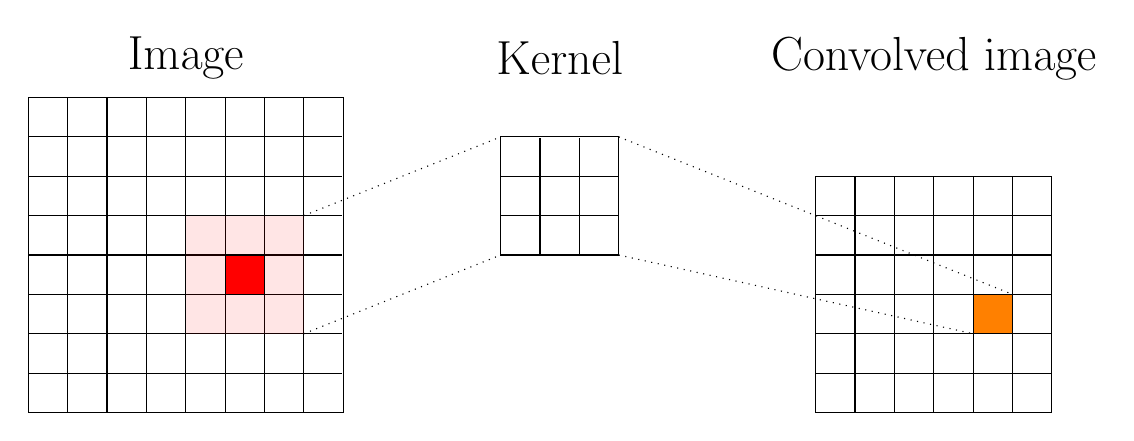
\begin{tikzpicture}
        
        \draw [fill=white] (0, 0) rectangle (4, 4);
        \draw [step=0.5] (0.01, 0.01) grid (3.99, 3.99);
        \node at (2, 4.5) {\LARGE Image};

        \draw [fill=white] (6, 2) rectangle (7.5, 3.5);
        \draw [step=0.5] (6.01, 2.01) grid (7.49, 3.49);
        \node at (6.75, 4.5) {\LARGE Kernel};

        \draw [fill=red, opacity=0.1] (2, 1) rectangle (3.5, 2.5);
        \draw [fill=red] (2.5, 1.5) rectangle (3, 2);
        
        \draw [fill=white] (10, 0) rectangle (13, 3);
        \draw [step=0.5] (10.01, 0.01) grid (12.99, 2.99);
        \node at (11.5, 4.5) {\LARGE Convolved image};
        
        \draw [fill=orange] (12, 1) rectangle (12.5, 1.5);

        \draw [dotted] (3.5, 2.5) -- (6, 3.5);
        \draw [dotted] (3.5, 1) -- (6, 2);
        \draw [dotted] (7.5, 3.5) -- (12.5, 1.5);
        \draw [dotted] (7.5, 2) -- (12, 1);

    \end{tikzpicture}

    \LARGE
    $$O = \sum_i \sum_j I_{i,j} K_{i,j}$$

    \normalsize
    See Lecture 4 for a refresher.
\end{frame}

\begin{frame}
    {Convolution terminology}
    Stride and padding
\end{frame}

\begin{frame}
    {What does a convolutional neural network learn?}
\end{frame}

\section{Building a CNN}

\begin{frame}
    {Convolutional layers}
    This is slide 3
\end{frame}

\begin{frame}
    {Pooling layers - max pooling}
\end{frame}

\begin{frame}
    {Pooling layers - average pooling}
\end{frame}

\begin{frame}
    {Putting it all together}
\end{frame}

\end{document}

